\documentclass[pdftex]{beamer}
\usepackage[british]{babel}
\usepackage{graphicx}
\usepackage{url}
\usepackage[normalem]{ulem}
\usepackage{tikz}

\mode<presentation>
\usetheme{Warsaw}
\useoutertheme{infolines}

\setbeamertemplate{navigation symbols}{}
% \usebeamertemplate*{logo}
% \logo{
\includegraphics[height=0.85cm]{../images/cmetlogo.png}}

\title[Measuring UK Crime Networks]{{\huge{Measuring UK Crime Networks}}}
\author[ASONAM 2014]{Giles Oatley and Tom Crick\\\url{tcrick@cardiffmet.ac.uk}}
\institute[@DrTomCrick]{Department of Computing \& Information
  Systems\\Cardiff Metropolitan University, UK\\\url{http://drtomcrick.com}}
\date{19 August 2014}

% logo  on title page only
\titlegraphic{
\includegraphics[width=4cm]{../images/cmetlogo.png}
}

\begin{document}

% titlepage
\begin{frame}
\titlepage
\end{frame}

% TOC
\section*{Talk Outline} 
\begin{frame} 
\tableofcontents 
\end{frame} 

\section{Introduction and Motivation}

\begin{frame}
\frametitle{Abstract}
{\small{{\emph{
This paper describes the output of a study to tackle the problem of
gang-related crime in the UK; we present the intelligence and
routinely gathered data available to a UK regional police force, and
describe an initial social network analysis of gangs in the Greater
Manchester area of the UK between 2000-2006.\newline

By applying social network analysis techniques, we attempt to detect
the birth of two new gangs based on local features (modularity,
cliques) and global features (clustering coefficient). Thus for the
future, identifying the changes in these can help us identify the
possible birth of new gangs (sub-networks) in the social
system.\newline

Furthermore, we study the dynamics of these networks globally and
locally, and have identified the global characteristics that tell us
that they are not random graphs -- they are small world graphs --
implying that the formation of gangs is not a random event. However,
we are not yet able to conclude anything significant about scale-free
characteristics due to insufficient sample size.}}}}
\end{frame}

\section{Gang Formation}

\begin{frame}
\frametitle{Gang Formation}
\begin{center}
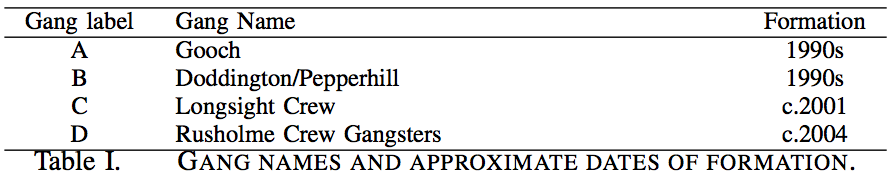
\includegraphics[width=0.8\textwidth]{../images/gangs.png}\newline\newline
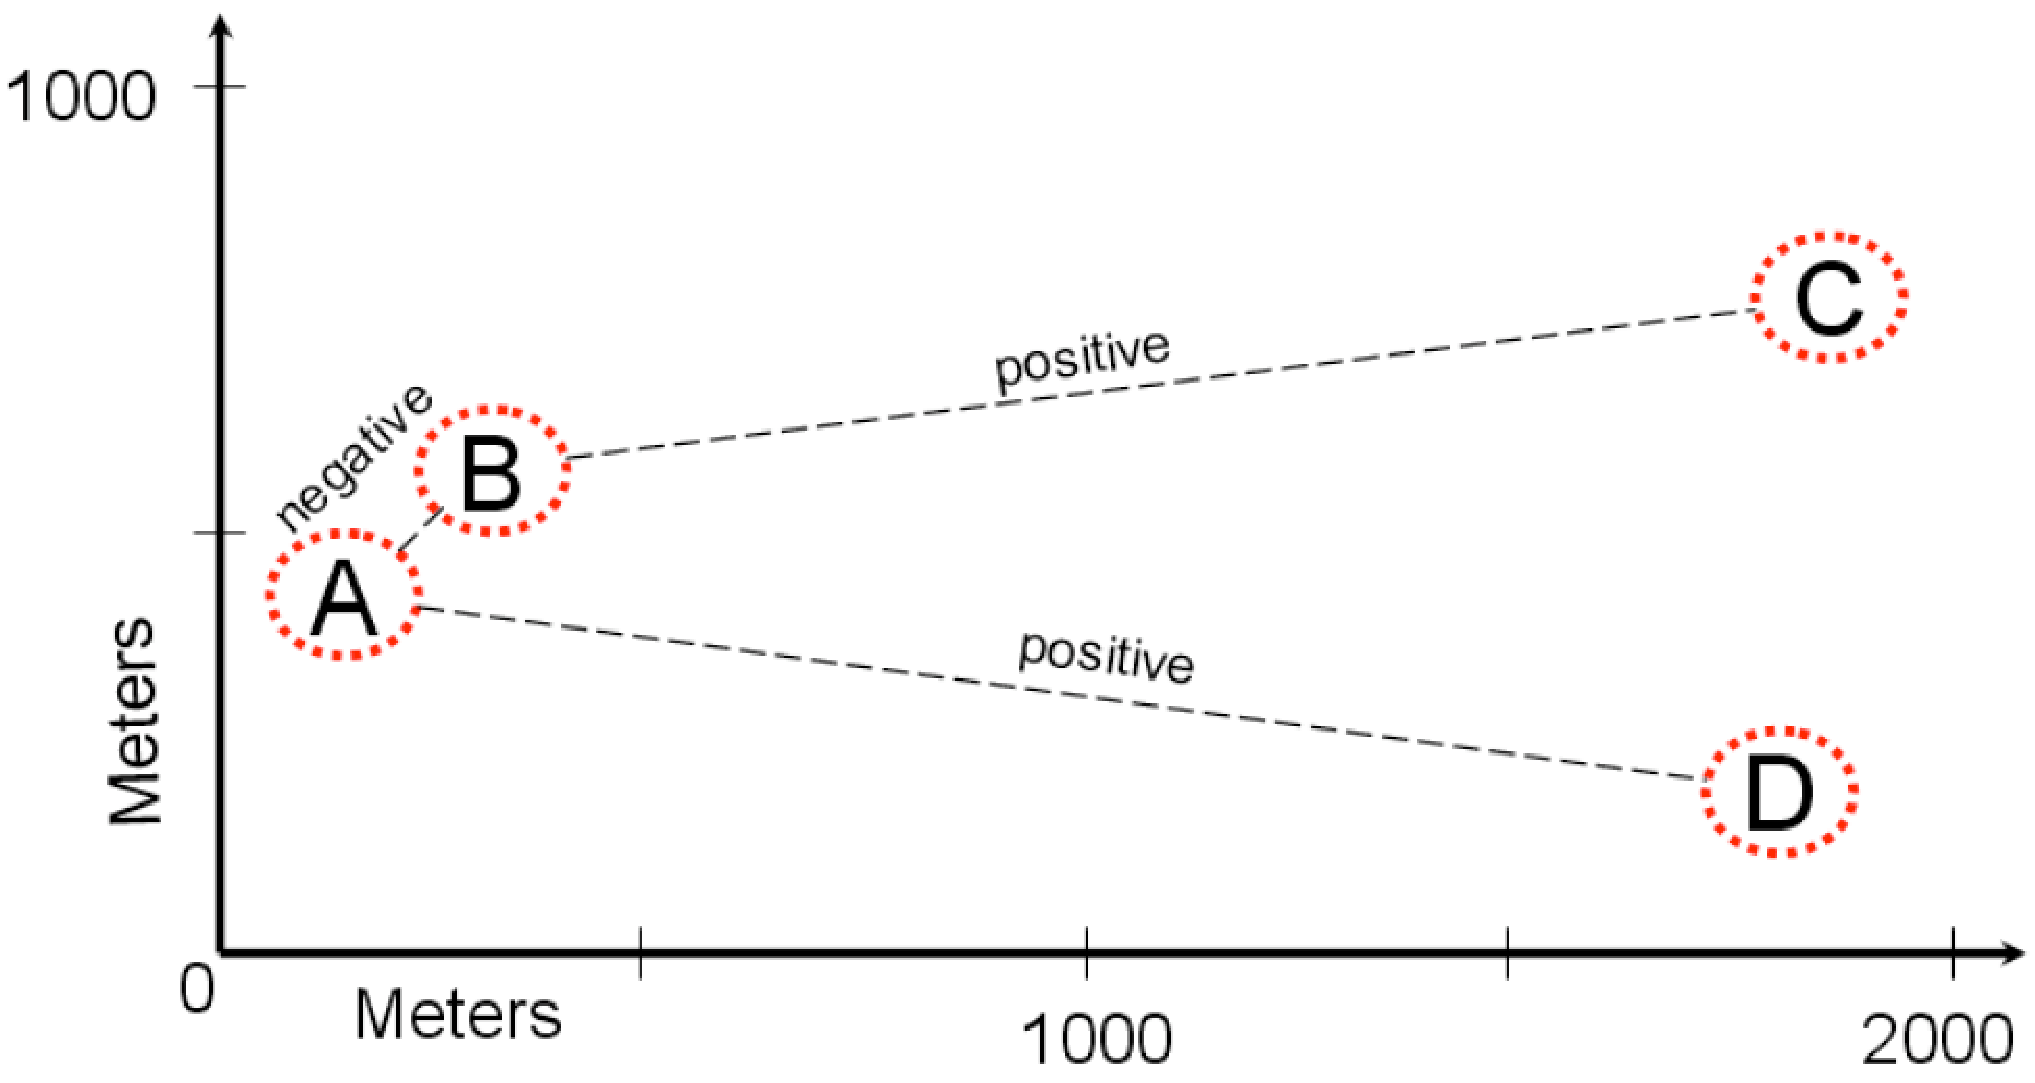
\includegraphics[width=0.7\textwidth]{../images/positive.pdf}
\end{center}
\end{frame}

\begin{frame}
\frametitle{Gang Formation}
\begin{center}
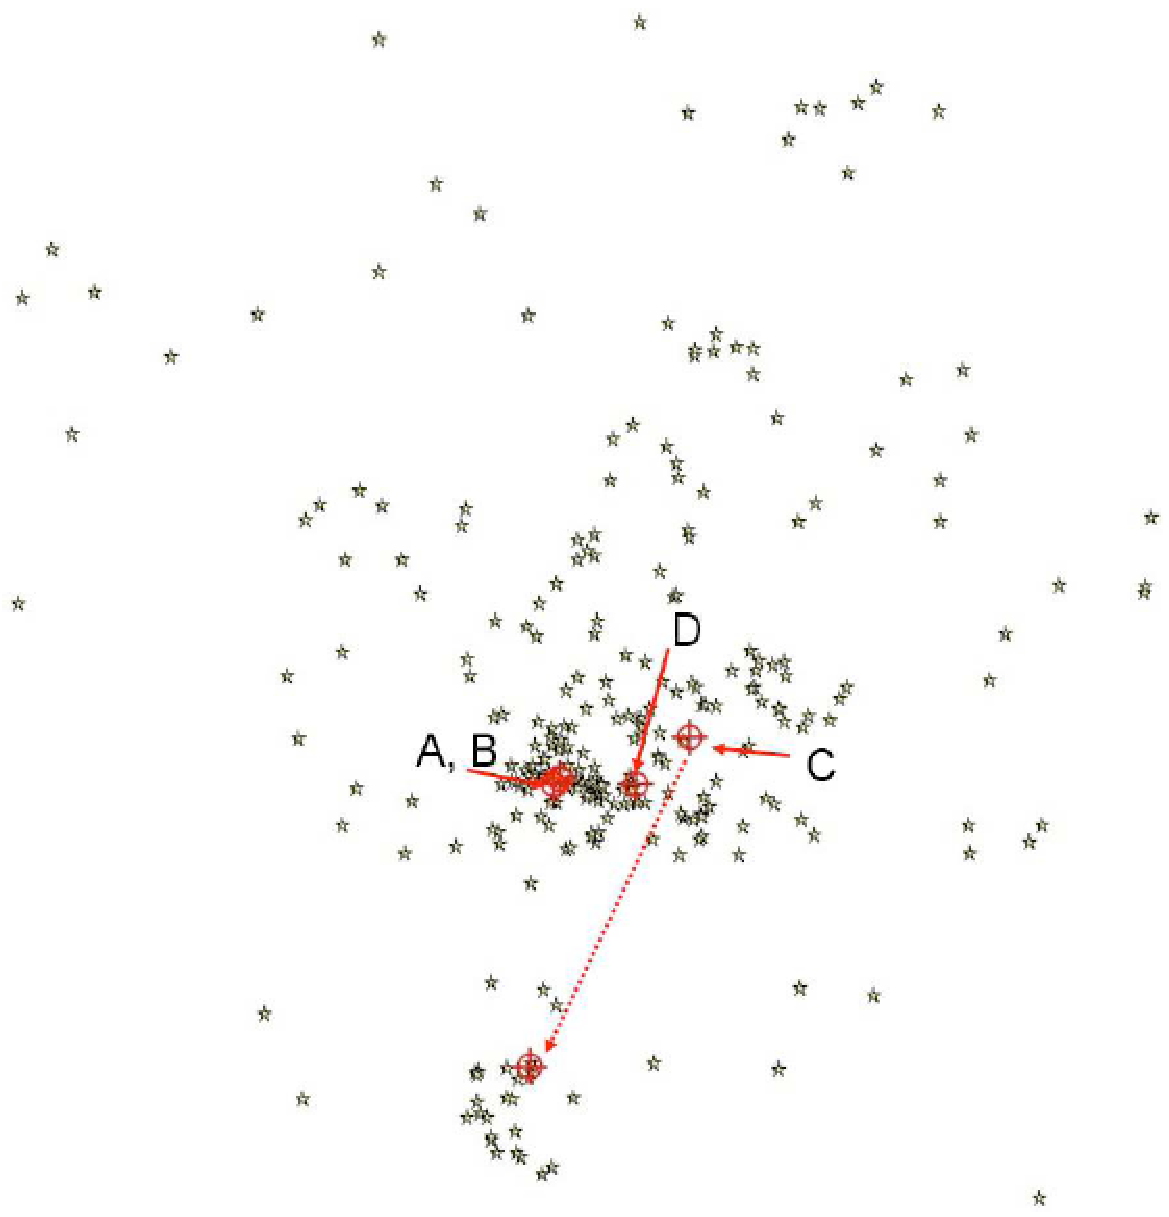
\includegraphics[width=0.5\textwidth]{../images/serious.pdf}
\end{center}
\end{frame}

\begin{frame}
\frametitle{Gangs in South Manchester, UK}
\begin{itemize}
\item All serious crimes: {\emph{murder, attempted murder, manslaughter,
  kidnapping, serious wounding, firearms offences}}. 
\item Gang C has moved into an additional location with drug selling.
\item 38\% ({\emph{n}}=162) of all serious crimes occurring within 1
  km radius (of gang locations).
\item 63\% of all serious crimes occur within 2 km.
\item 53\% ({\emph{n}}=9) of murders are within 3 km
\item 38\% ({\emph{n}}=34) of attempted murders are within 1 km, 63\% within 2 km
\item 33\% ({\emph{n}}=17) of serious woundings are within 1 km, 48\% are within 2 km. 
\end{itemize}
\end{frame}

\section{Police Databases}

{ % all template changes are local to this group.
    \setbeamertemplate{navigation symbols}{}
    \begin{frame}[plain]
        \begin{tikzpicture}[remember picture,overlay]
            \node[at=(current page.center)] {
                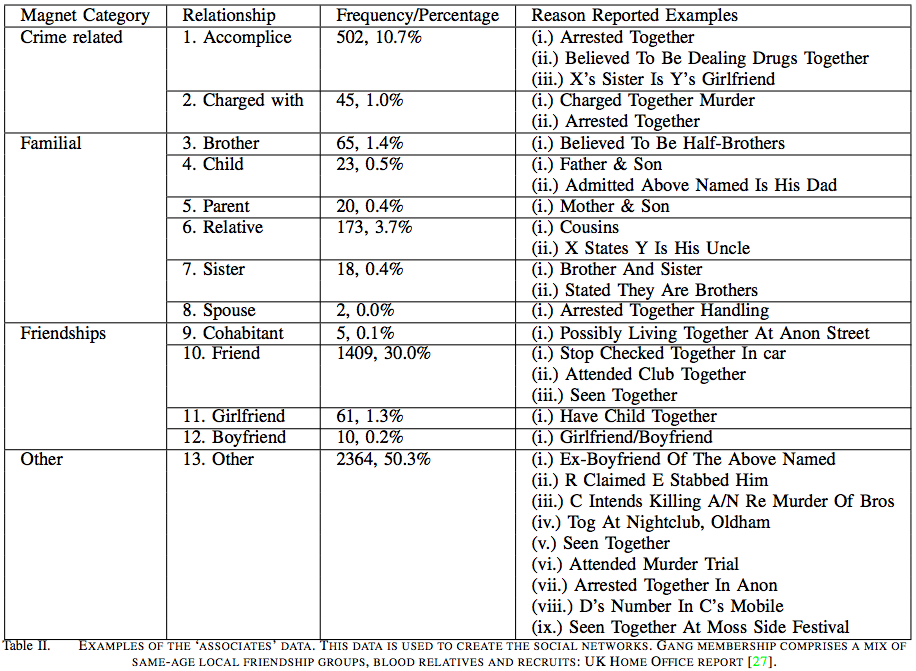
\includegraphics[width=0.9\paperwidth]{../images/associatesdata.png}
            };
        \end{tikzpicture}
     \end{frame}
}

\section{Network Characterisation}

\begin{frame}
\begin{center}
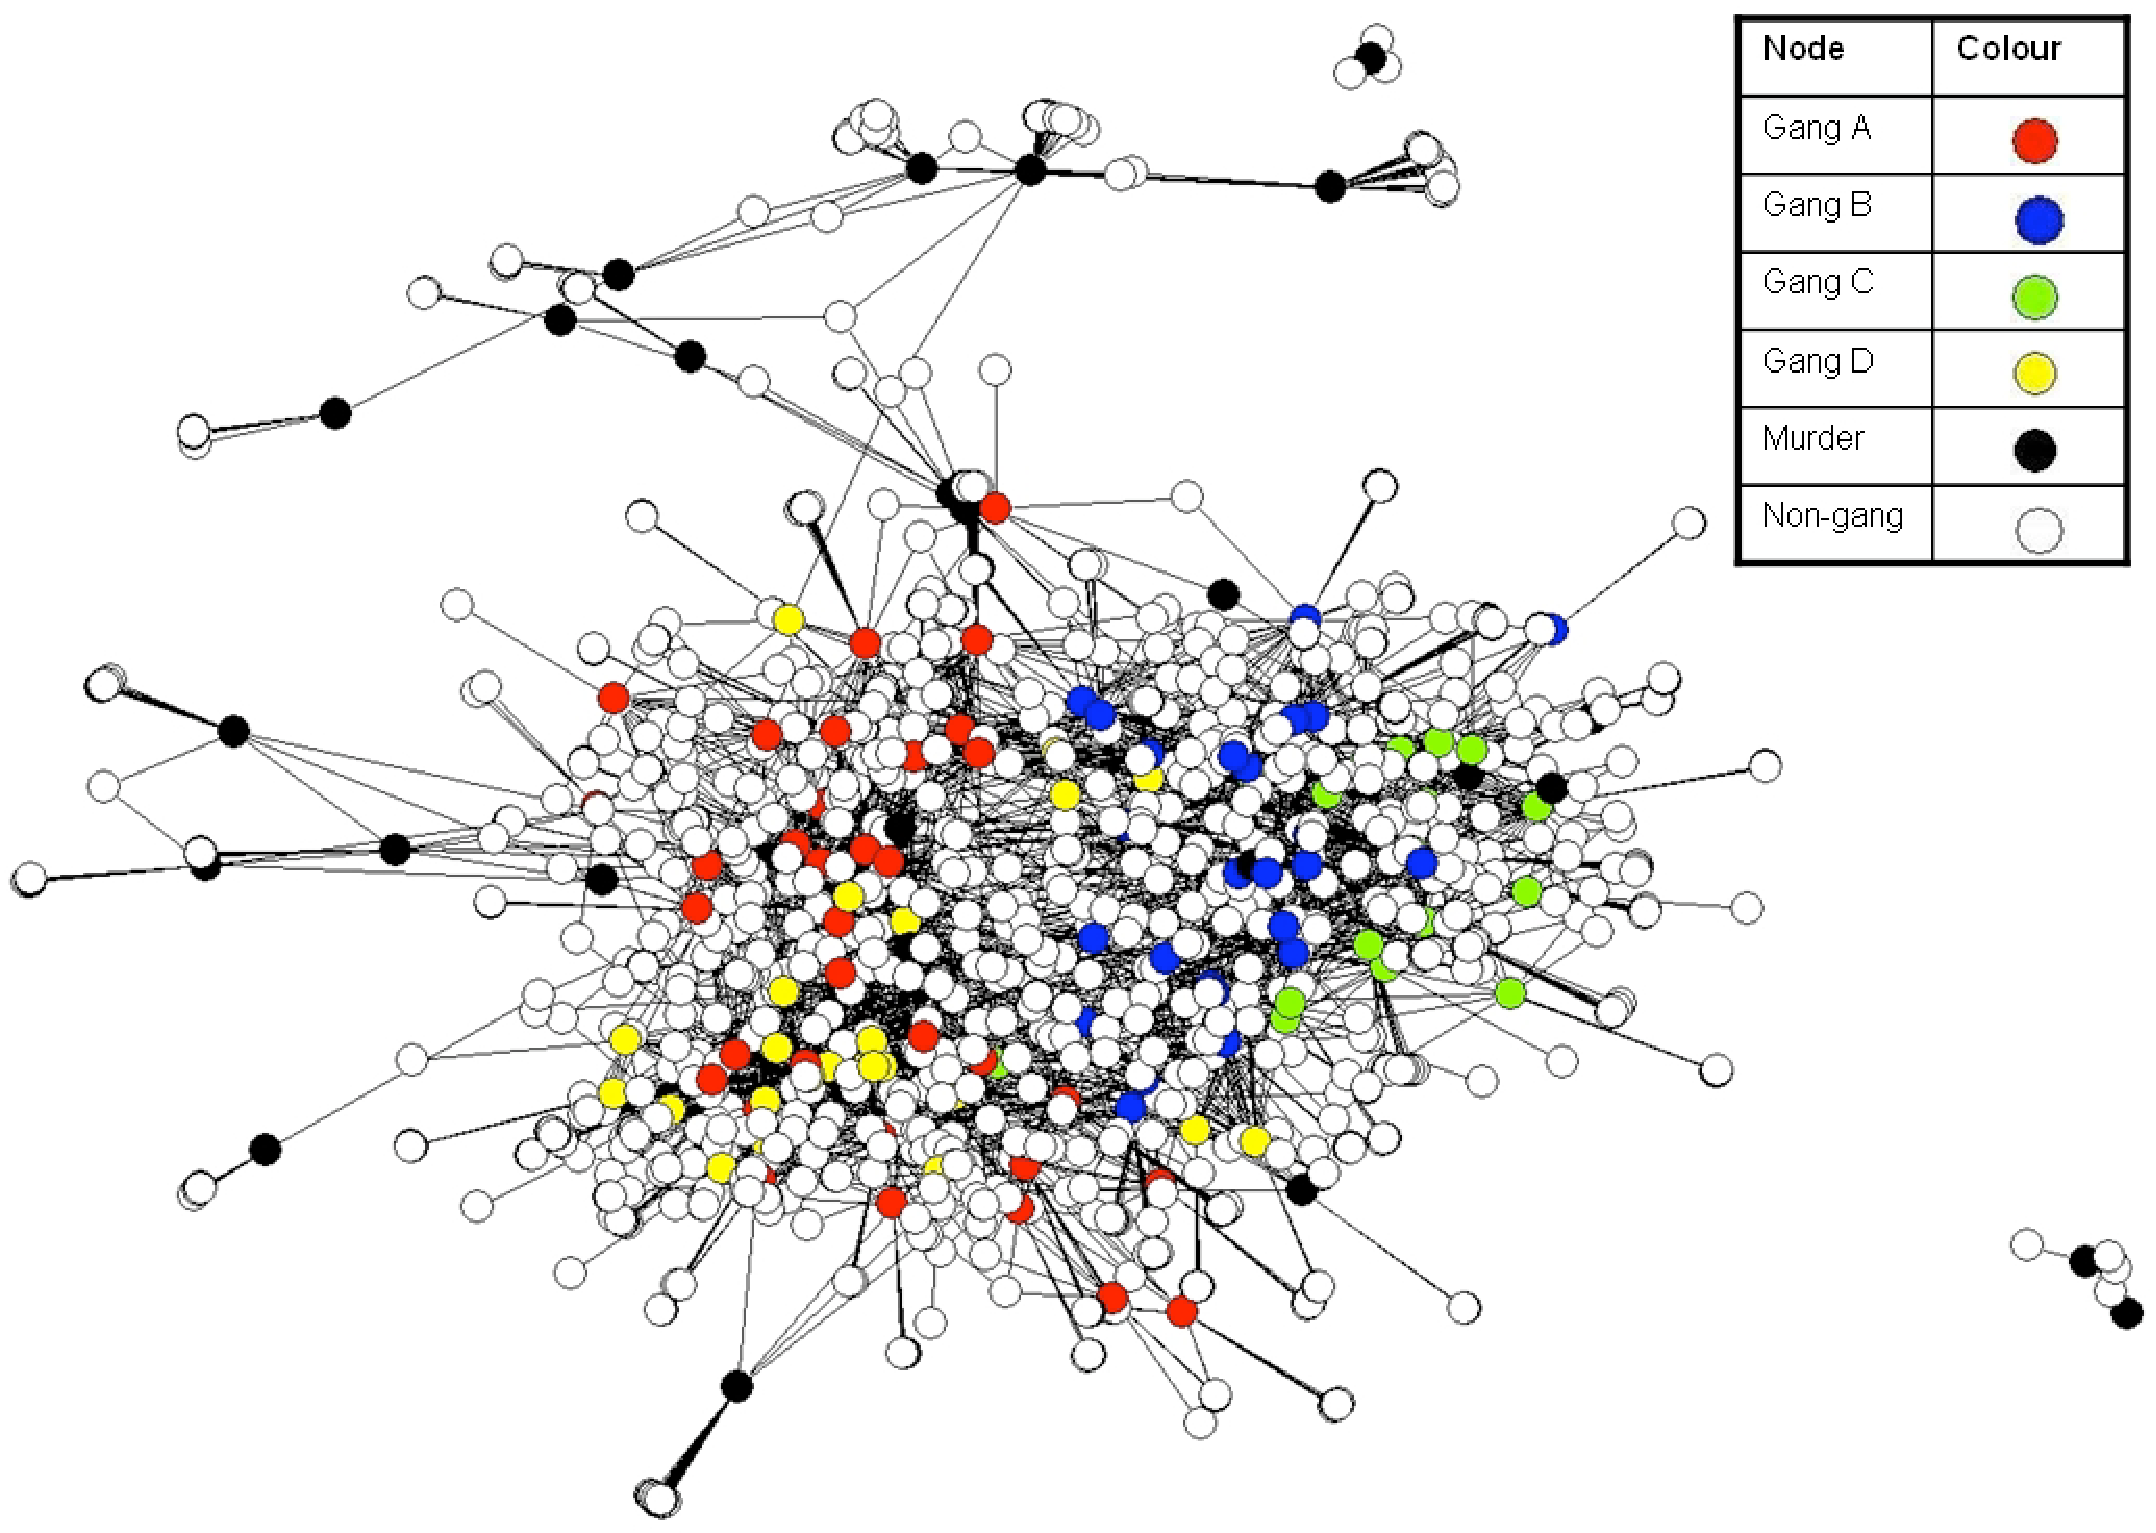
\includegraphics[width=0.7\paperwidth]{../images/legend2006.pdf}
\end{center}
\hfill\scriptsize{{\textbf{Network in 2006.}}}
\end{frame}

\begin{frame}
\begin{center}
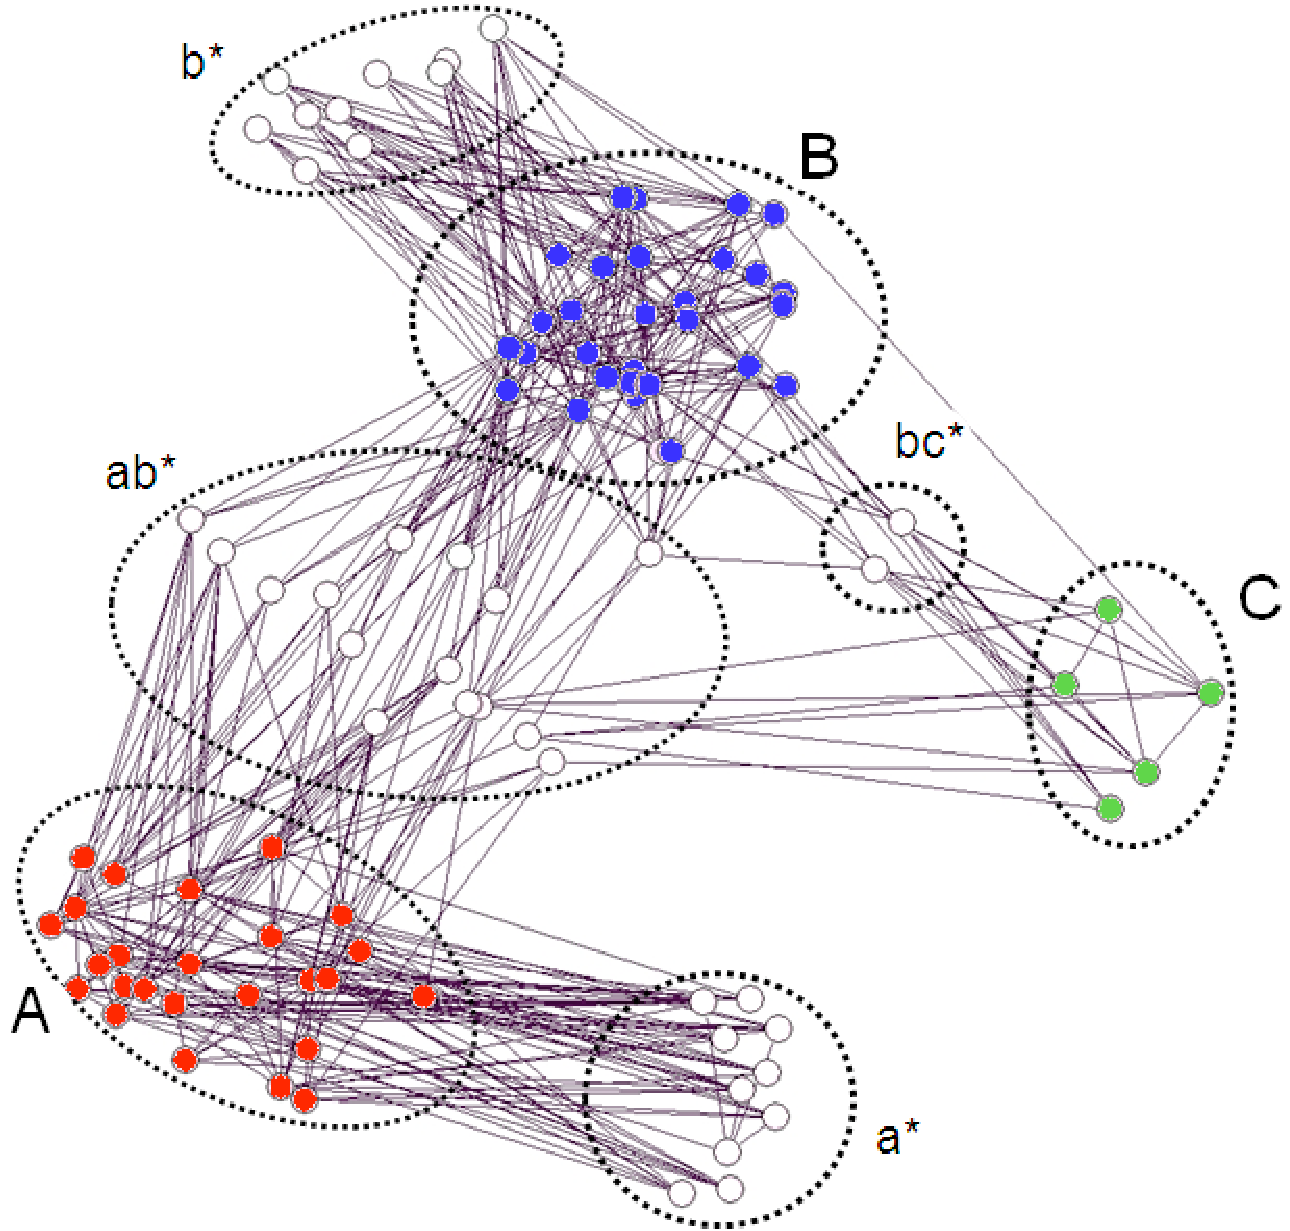
\includegraphics[width=0.6\paperwidth]{../images/2002core_labelled.pdf}
\end{center}
\scriptsize{{\textbf{Link reduction, showing Gangs A and B and emergence of Gang
C (for 2002).}} This also illustrates the large amount of non-gang members who
are associated with individual gangs ({\emph{a*, b*}}) or who are intermediaries ({\emph{ab*,
bc*}}).}
\end{frame}

\subsection{Small-World}

\begin{frame}
\frametitle{Small-World}
\begin{itemize}
\item A small-world network has both local connectivity and global reach, and is a simple connected graph {\emph{G}} exhibiting two properties:
\begin{enumerate}
\item Small characteristic path length: the presence of short-cut
  connections between some vertices results in a small characteristic
  path length {\emph{L(G)}}.
\item Large clustering coefficient: each vertex of {\emph{G}} is linked to a
  relatively well-connected set of neighbouring vertices, resulting in
  a large value for the clustering coefficient {\emph{C(G)}}.
\end{enumerate}
\pause
\item To determine whether our network is a random one or is
  small-world, we can test whether or not it has exponential
  {\emph{k}}-connectivity distribution.
\pause
\item {\textbf{We do not observe this in the data}}, however, we do see large
  clustering coefficients, and the average path lengths are always
  less than {\emph{log(n)}}. 
\item {\textbf{Based upon these two criteria we can still conclude that our
  networks have small-world characteristics.}}
\end{itemize}
\end{frame}

\subsection{Scale-Free}

\begin{frame}
\frametitle{Scale-Free}
\begin{itemize}
\item Plotting the clustering coefficient as a function of the number
  of nodes {\emph{n}}, should follow the power-law distribution for scale-free
  networks, with the clustering coefficient being roughly four times
  larger than random networks.
\item The value of the clustering coefficient for a random networks
  will be {\emph{1/n}}. 
\pause
\item We compare the values of {\emph{4/n}} against {\emph{CC}}.
\item  As the cumulative links increase from 2000 to 2006, the value
  of {\emph{CC}} generally increases (with the number of nodes {\emph{n}}) and is always
  significantly higher than the values of {\emph{4/n}}. 
\item Each of the gang values for {\emph{CC}} are also significantly higher
  than would be expected in a random network.
\end{itemize}
\end{frame}

\begin{frame}
\frametitle{Scale-Free cont.}
\begin{itemize}
\item The diameter of the network (longest path length) should be
  approximately {\emph{log(log(n))}} for scale-free networks.
\begin{itemize}
\item {\textbf{In both cases (for the gangs and the years) the real values are
  significantly higher than would be expected for a scale-free
  network.}}
\end{itemize}
\pause
\item The average path length should be approximately {\emph{log(n)}} for
  scale-free networks. 
\begin{itemize}
\item {\textbf{For both the gangs and years data it was actually smaller
  than {\emph{log(n)}}, indicating scale-free networks.}}
\end{itemize}
\pause
\item The statistics on degree centrality were low, indicating that
  there is no group leader. 
\item As we know when Gangs C (2001) and D (2004) are formed, it is
  interesting to note that the characteristic of the networks at this
  time are that the betweenness centralisation reaches 0.2.
\item It is necessary to compare the closeness and betweenness
  averages for each gang against the value for the overall network.
\end{itemize}
\end{frame}

\subsection{Power Law Investigation}

\begin{frame}
\frametitle{Power Law Investigation}
\begin{center}
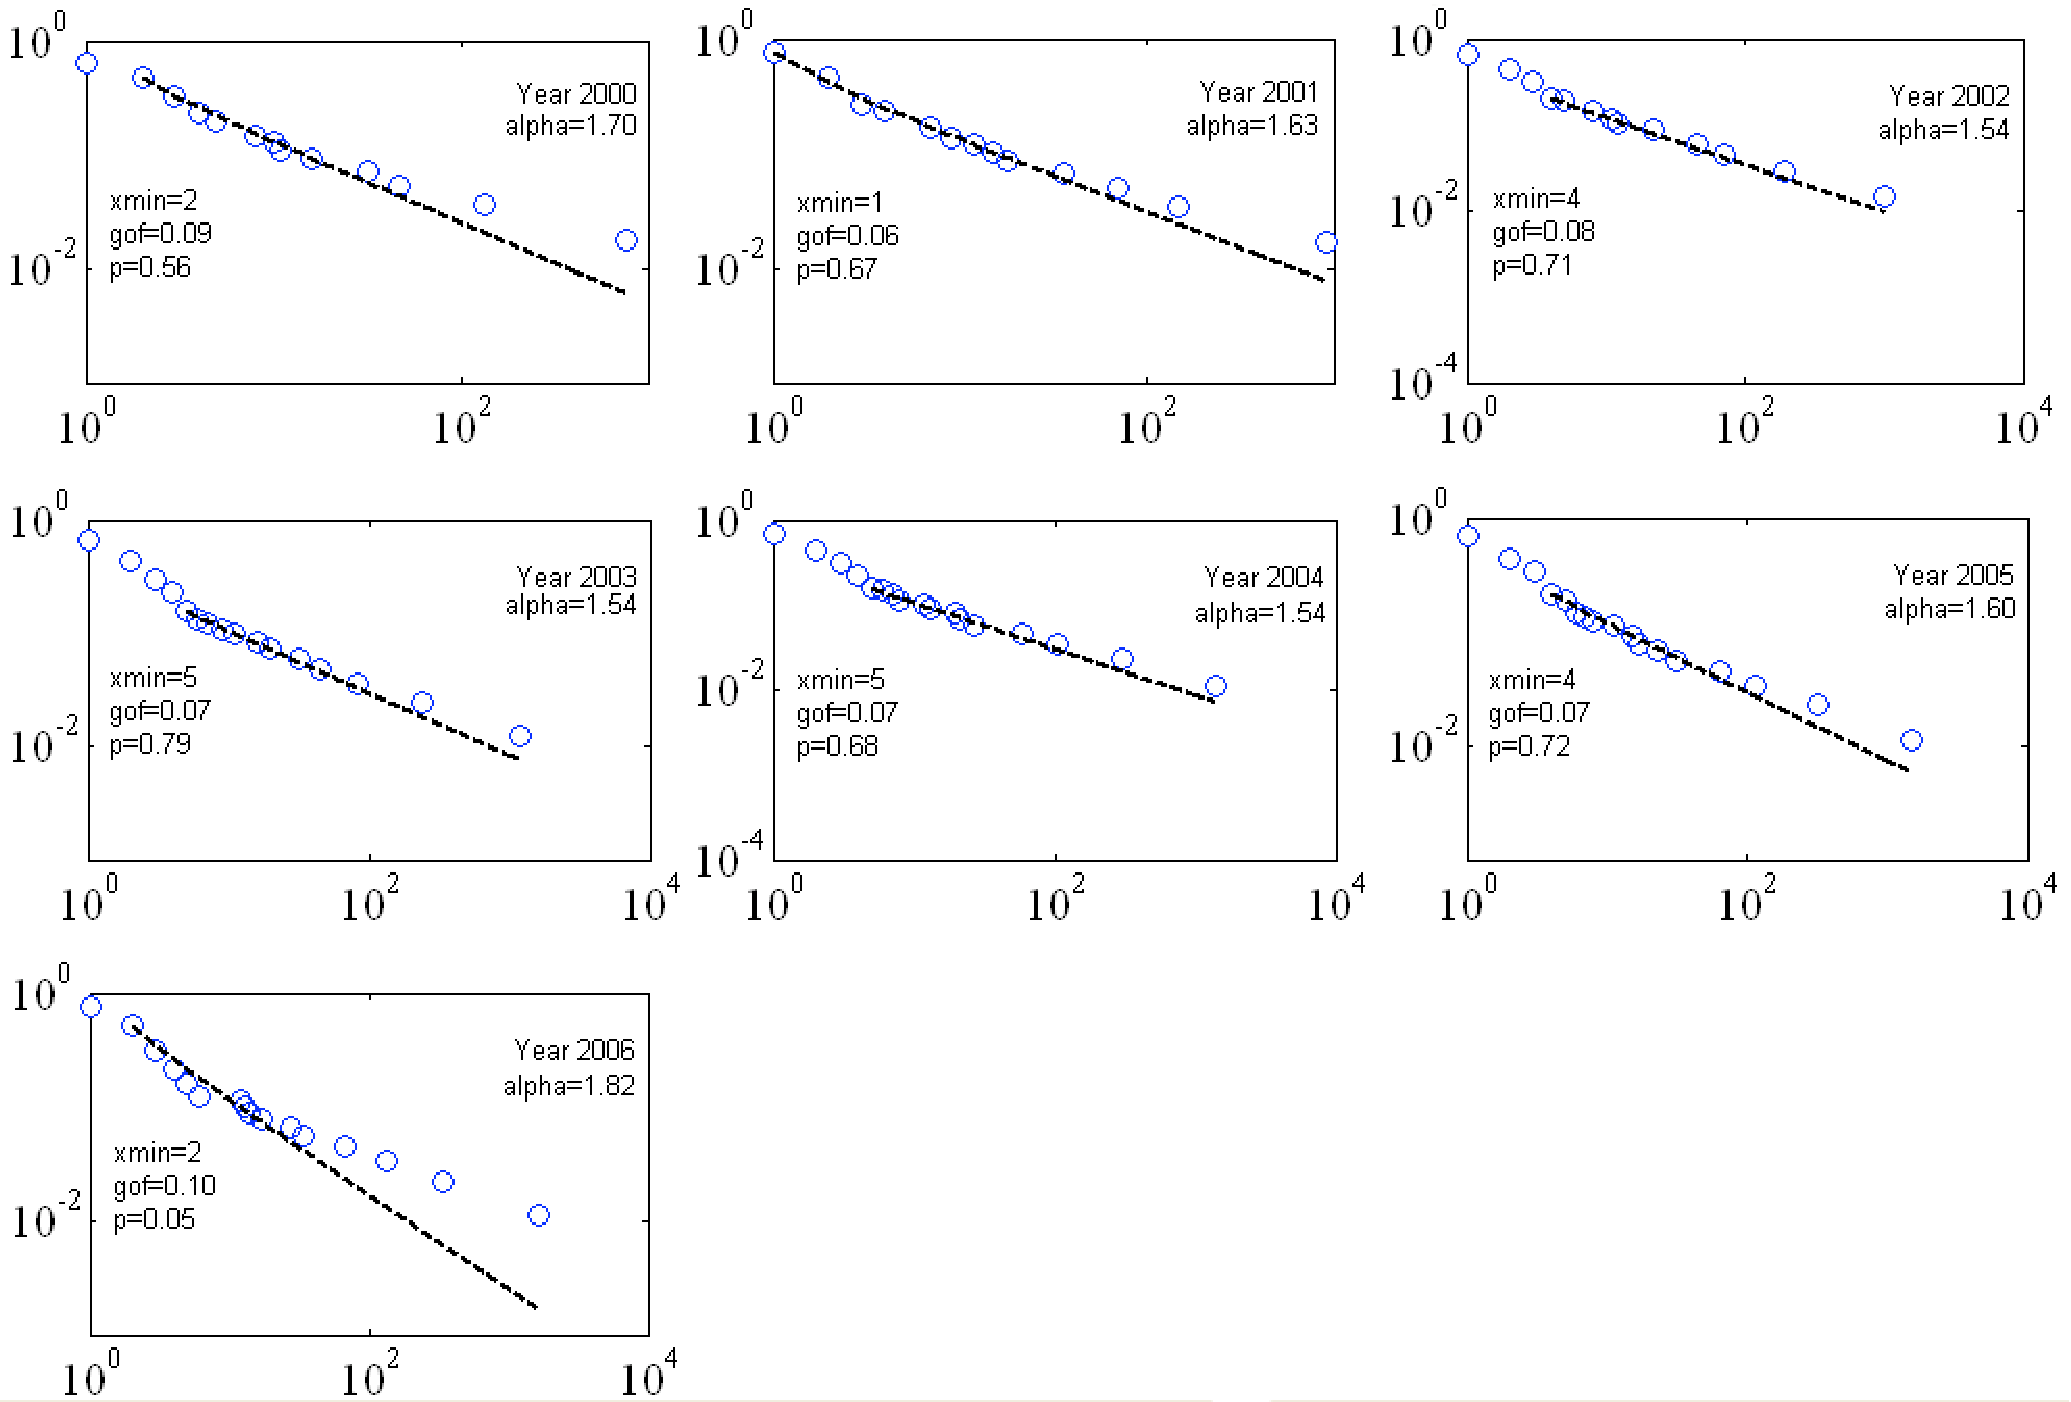
\includegraphics[width=0.9\paperwidth]{../images/clausetcumulative.pdf}
\end{center}
\end{frame}

\subsection{Emergence of Gangs}

\begin{frame}
\begin{center}
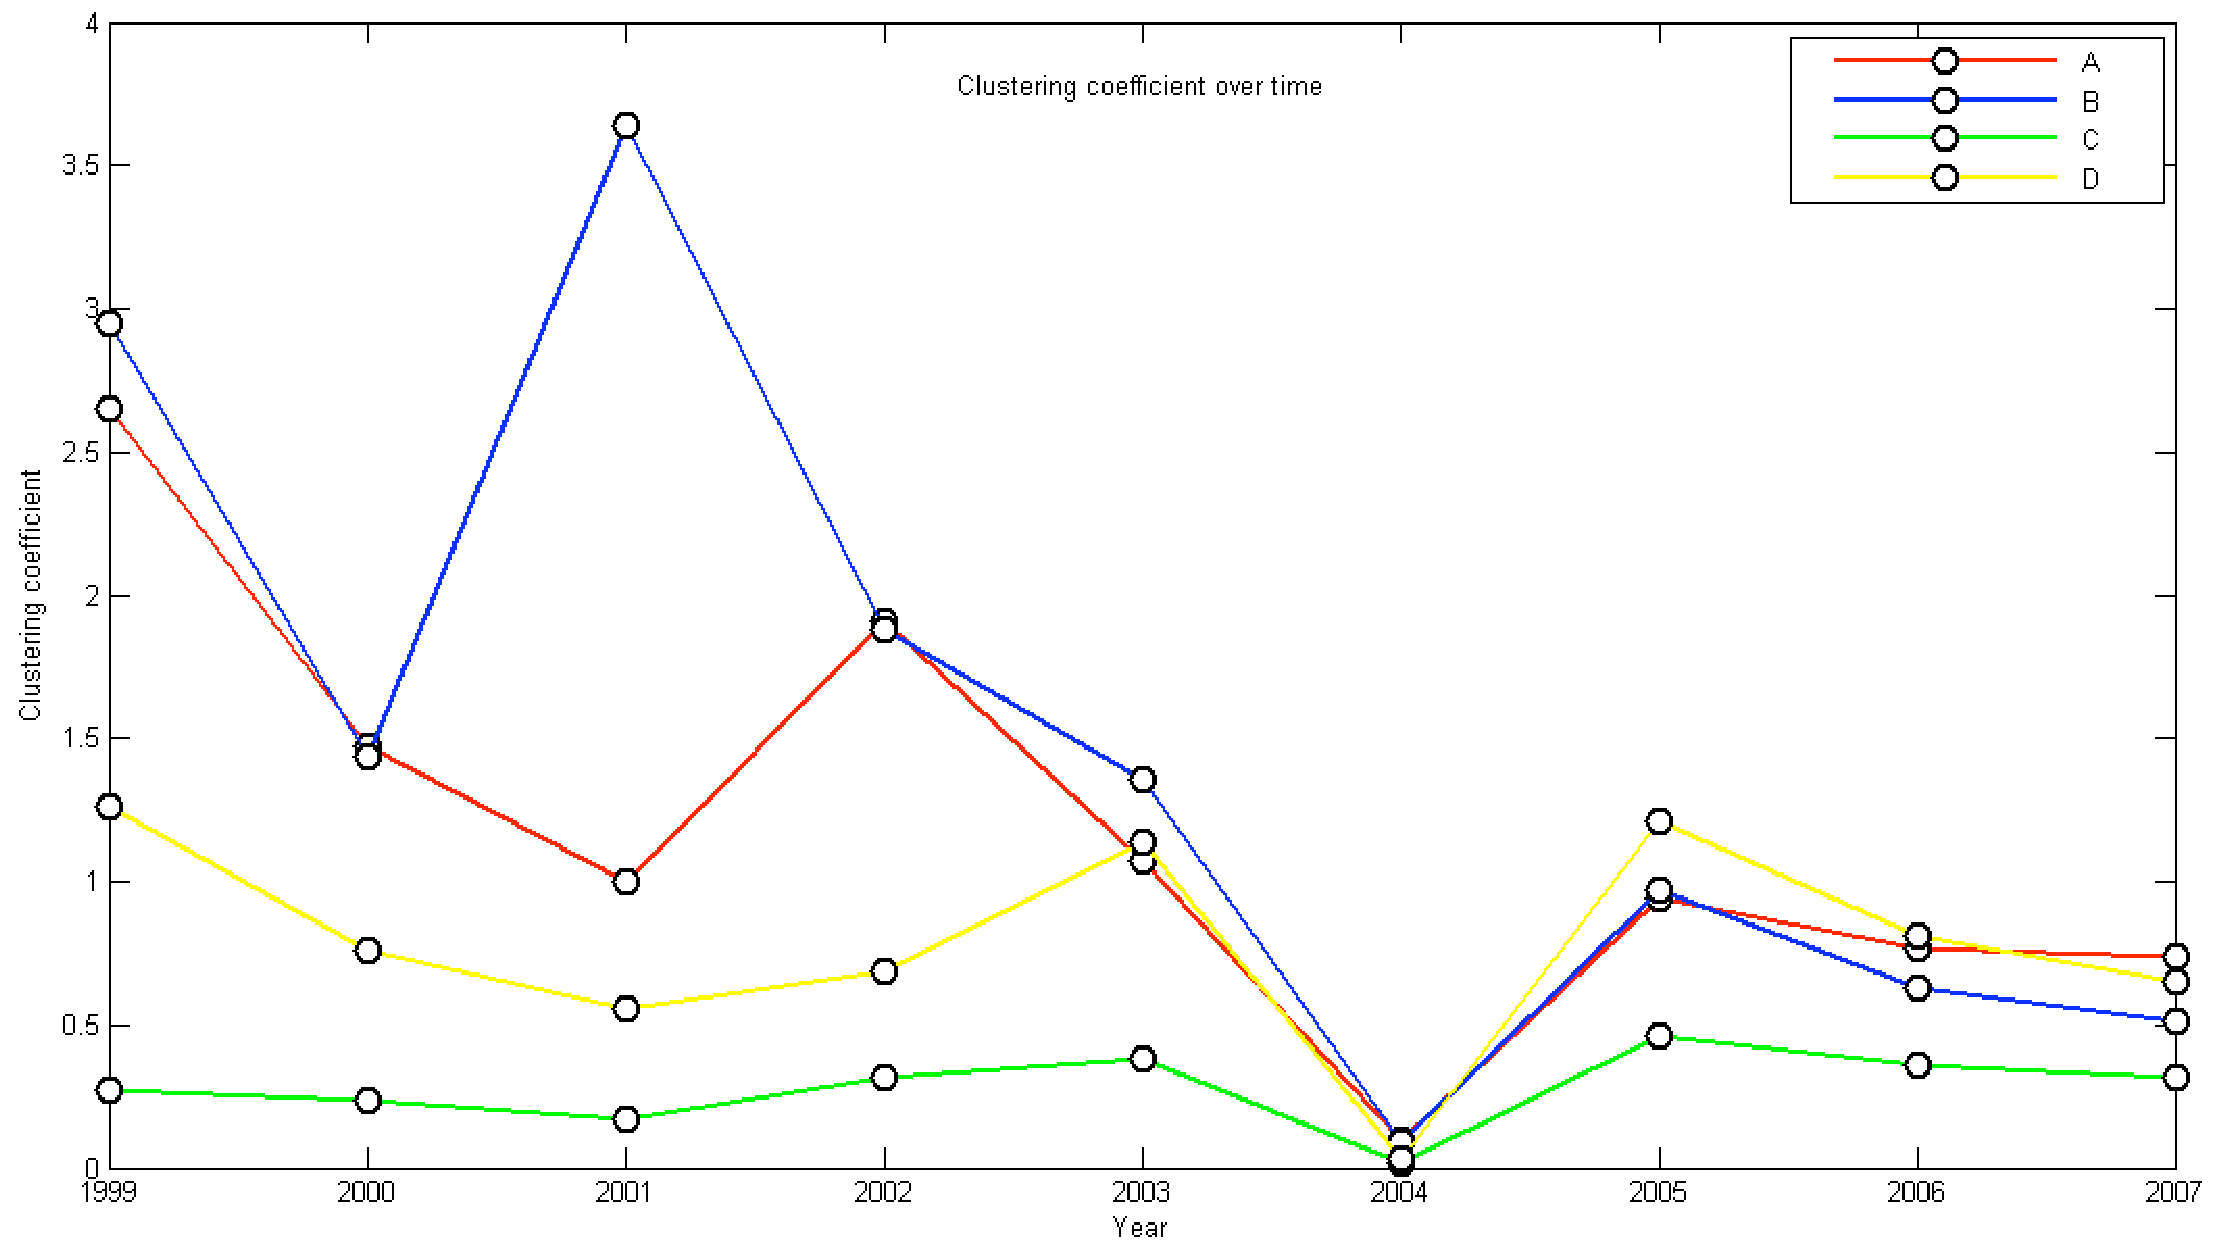
\includegraphics[width=0.9\paperwidth]{../images/gangscc1years.pdf}
\end{center}
\scriptsize{{\textbf{Per year clustering coefficients for each gang.}} Gang C was formed
in 2001, Gang D in 2004.}
\end{frame}

\begin{frame}
\begin{center}
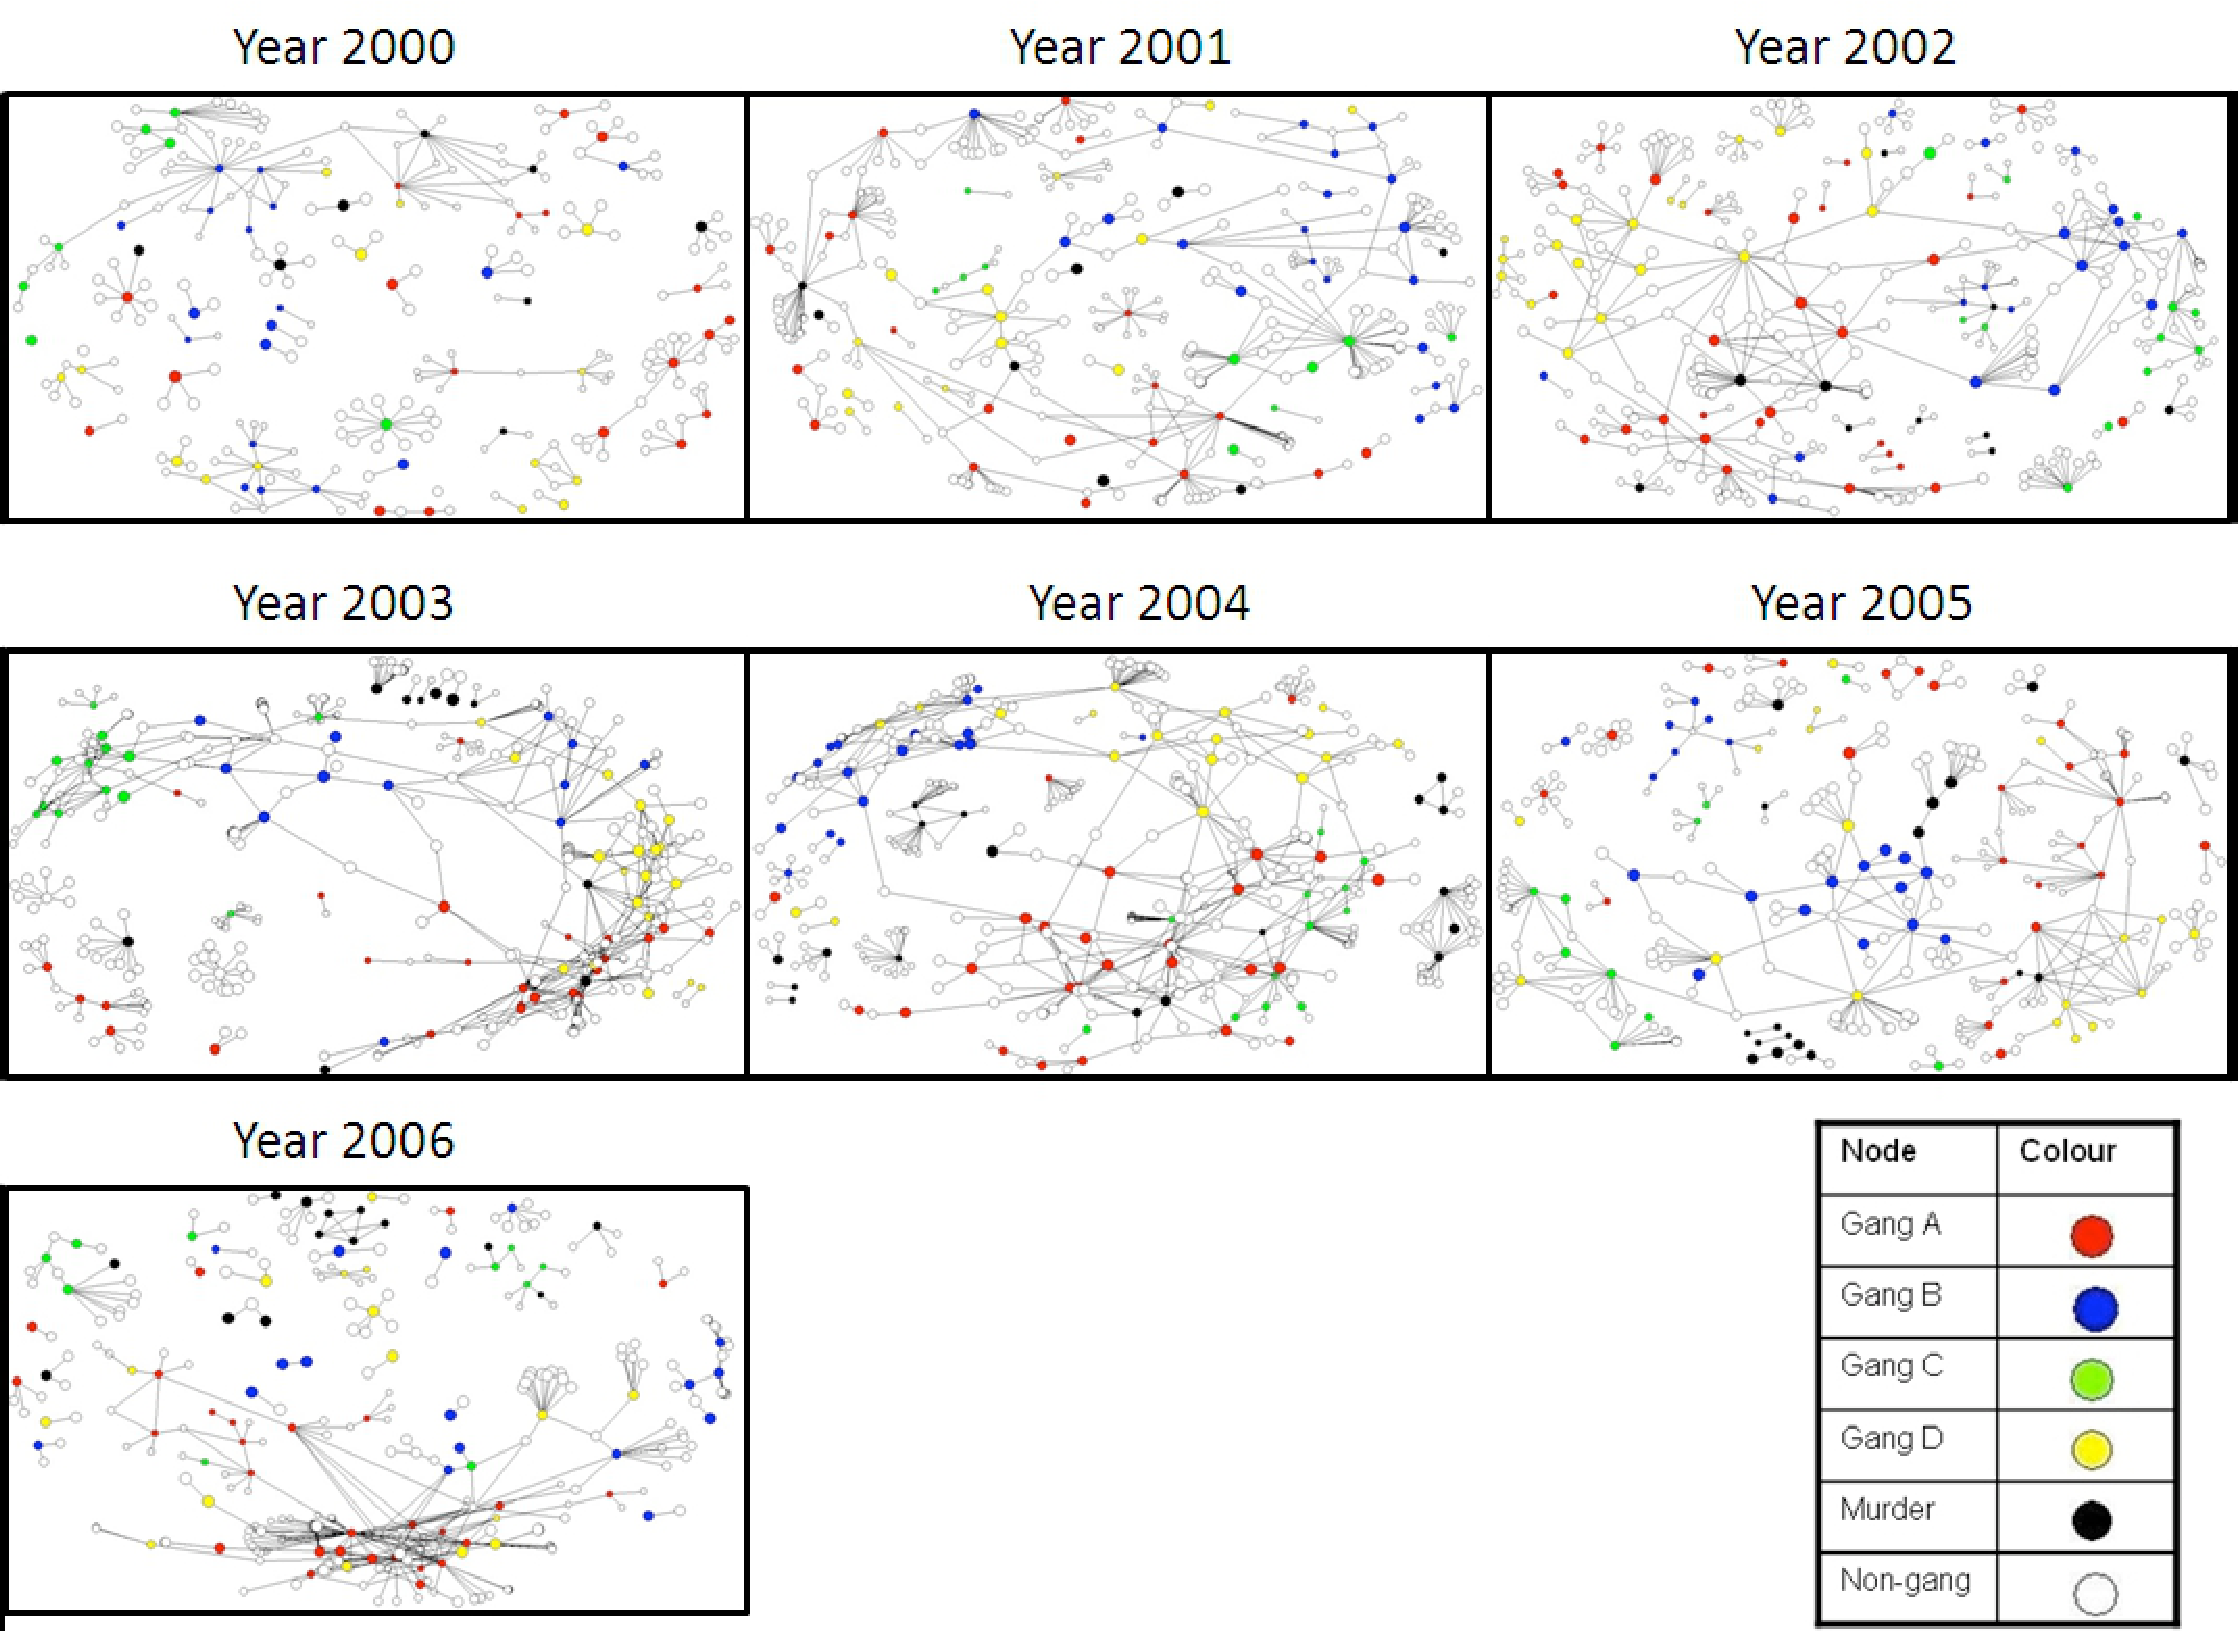
\includegraphics[width=0.8\paperwidth]{../images/all.pdf}
\end{center}
\scriptsize{{\textbf{Annual links formation.}} Only nodes directly
  connected to a gang member are included.}
\end{frame}

\section{Conclusions and Future Work}

\begin{frame}
\frametitle{Conclusions}
\begin{itemize}
\item Identifying changes can help us identify the possible birth of
  new gangs (sub-networks) in the social system.
\item Through studying the dynamics of these networks globally and
  locally, we have identified the global characteristics that tell us
  that they are not random graphs -- they are small-world graphs -- 
  implying that the formation of gangs is not a random event. 
\item However, we are not yet able to conclude anything significant
  about scale-free characteristics due to insufficient sample size.
\end{itemize}
\end{frame}

\begin{frame}
\frametitle{Future Work}
\begin{itemize}
\item Further pre-processing of original data is being carried out.
\item The quality of the data collection process is to be improved.
\item Criminal behaviour (modus operandi and offence profiling) is to
be incorporated into the social network analysis.
\pause
\item {\textbf{There is significant future work available with this dataset.}}
\end{itemize}
\end{frame}

\begin{frame}
\frametitle{Acknowledgements}
\begin{itemize}
\item Acknowledgements:
\begin{itemize}
\item UK EPSRC Sandpit on Gun Crime
\item Xcalibre Task Force, Greater Manchester Police, UK\newline
\end{itemize}
\item Papers and presentations:
  \url{https://github.com/tomcrick/ASONAM2014}\\
\url{https://github.com/tomcrick/FOSINT-SI2014}\newline
\item Contact: \url{http://drtomcrick.com}
\end{itemize}
\end{frame}

\end{document}
